\subsection{Local environment and structural response}

We next examine local Pt coordination before and after
\ce{CO} adsorption, followed by the optimized \ce{Pt-C} distances and
electron densities at the Pt--C bond critical points.

\subsubsection{Local Pt coordination before and after CO adsorption}
\label{subsec:local_pt_coordination}

We use Hoppe's effective coordination number (ECoN) to describe the
local environment of each Pt adsorption site, separating the contributions
from neighboring Pt and Ge atoms. The descriptors are first evaluated for the
bare clusters and then for the optimized carbonyl complexes, allowing us to compare the
initial site environment with its change upon CO adsorption.


{For the pure-Pt clusters, $ECoN_{\rm total}^{0}=ECoN_{\rm Pt}^{0}$.
The initial ECoN values for \ce{Pt10^{GM}} and \ce{Pt10^{der}} are given in
Supporting Table~\ref{tab:tfg_pt10_bare_econ}.
The two groups of Pt sites in the nonet \ce{Pt10^{GM}} have different initial
coordination but give almost identical binding energies. The six more highly
coordinated sites, with $ECoN^{0}$ close to 5.68, give
$BE_{\rm ad}(\ce{CO})=-1.60$ eV, while the four sites with $ECoN^{0}$ close
to 3.00 give $-1.58$ eV. Thus, the
large difference in initial coordination is accompanied by only a small
difference in CO binding within this nonet series.}

{Hossain and co-workers found that \ce{CO} preferentially adsorbs at
less coordinated sites on Pt nanoparticles.\cite{hossain:lowcoord:2020}
The triplet \ce{Pt10^{der}} shows this tendency.
The most highly coordinated initial sites,
1 and 9, converge to the weakest-binding minimum ($-2.16$ eV), whereas site
6, with lower initial coordination, gives the strongest binding ($-2.66$ eV).
{Sites 8 and 10 illustrate the effect of structural relaxation:} although their initial
$ECoN^{0}$ values are 3.03 and 4.54, respectively, both relax to the same
carbonyl minimum, with a final $ECoN^{\ce{CO}}$ of 4.97 and a binding energy
of $-2.65$ eV
(Supporting Table~\ref{tab:tfg_pt10_der_econ_co}).}

For Pt–Ge clusters, we further examine whether CO binding depends not only on the coordination of the adsorption site but also on the chemical identity of its neighboring atoms. We distinguish the effective contributions of Pt and Ge neighbors through $ECoN_{\rm Pt}^{0}$ and $ECoN_{\rm Ge}^{0}$, respectively, and define $x_{\rm Ge}^{0}$ as the fraction of the initial total coordination arising from Ge neighbors.

\begin{table}[htbp]
\caption{Local Hoppe ECoN descriptors for each Pt adsorption site in the bare
\ce{Pt10}-to-\ce{Pt-Ge} clusters, before \ce{CO} is added. The superscript 0
denotes this pre-adsorption geometry. Only metal neighbors are included, and
$ECoN_{\rm total}^{0}=ECoN_{\rm Pt}^{0}+ECoN_{\rm Ge}^{0}$ and
$x_{\rm Ge}^{0}=ECoN_{\rm Ge}^{0}/ECoN_{\rm total}^{0}$. Paired labels denote
initial positions represented by the same listed descriptors and adsorption
result. Sites 5 and 7 of \ce{Pt4Ge6CO} are listed separately because their
initial ECoN descriptors differ, although they converge to the same carbonyl
minimum.}
\label{tab:tfg_crossed_ptge_econ_descriptors}
\small
\begin{adjustbox}{max width=\linewidth}
\begin{tabular}{lcrrrrr}
\toprule
{System} &  {Site} & {$BE_{\rm ad}(\ce{CO})$ / eV} &
{$ECoN_{\rm total}^{0}$} & {$ECoN_{\rm Pt}^{0}$} & {$ECoN_{\rm Ge}^{0}$} &
{$x_{\rm Ge}^{0}$} \\
\midrule
\ce{Pt6Ge4^{der}CO}  & 2  & -2.25 & 3.22 & 1.88 & 1.34 & 0.42 \\
\ce{Pt6Ge4^{der}CO}  & 9  & -2.25 & 2.92 & 0.73 & 2.19 & 0.75 \\
\ce{Pt6Ge4^{der}CO}  & 1/4  & -2.24 & 4.60 & 2.70 & 1.90 & 0.41 \\
\ce{Pt6Ge4^{der}CO}  & 5/7  & -1.57 & 2.77 & 0.53 & 2.24 & 0.81 \\
\midrule
\ce{Pt5Ge5^{der}CO}  & 6/8  & -2.08 & 5.58 & 1.42 & 4.16 & 0.75 \\
\ce{Pt5Ge5^{der}CO}  & 7/10 & -1.66 & 2.91 & 0.74 & 2.17 & 0.75 \\
\ce{Pt5Ge5^{der}CO}  & 4  & -1.34 & 2.95 & 0.00 & 2.95 & 1.00 \\
\midrule
\ce{Pt4Ge6^{der}CO}  & 5  & -1.46 & 3.99 & 0.56 & 3.43 & 0.86 \\
\ce{Pt4Ge6^{der}CO}  & 7  & -1.46 & 3.48 & 0.28 & 3.20 & 0.92 \\
\ce{Pt4Ge6^{der}CO}  & 2  & -1.31 & 4.71 & 0.47 & 4.25 & 0.90 \\
\ce{Pt4Ge6^{der}CO}  & 1  & -1.05 & 4.41 & 0.09 & 4.32 & 0.98 \\
\bottomrule
\end{tabular}
\end{adjustbox}
\end{table}

For \ce{Pt6Ge4^{der}} (Table~\ref{tab:tfg_crossed_ptge_econ_descriptors}), site 5/7 has the largest initial Ge fraction ($x_{\rm Ge}^{0}=0.81$) and the weakest CO binding ($BE_{\rm ad}(\ce{CO})=-1.57$ eV). Sites 2 and 1/4 have smaller initial Ge fractions and are among the strongest-binding sites. Site 9 is also among the strongest-binding sites ($-2.25$ eV), despite its relatively high initial Ge fraction ($x_{\rm Ge}^{0}=0.75$); its binding energy is nearly the same as those of sites 2 and 1/4 ($-2.25$ and $-2.24$ eV). Upon CO adsorption, site 9 shows a larger change in its local descriptors than site 5/7: \textcolor{purple}{$ECoN_{\rm Pt}^{0}=0.73$} increases to \textcolor{purple}{$ECoN_{\rm Pt}^{\ce{CO}}=1.16$} and \textcolor{purple}{$x_{\rm Ge}^{0}=0.75$} decreases to \textcolor{purple}{$x_{\rm Ge}^{\ce{CO}}=0.61$}, compared with changes from \textcolor{purple}{$ECoN_{\rm Pt}^{0}=0.53$} to \textcolor{purple}{$ECoN_{\rm Pt}^{\ce{CO}}=0.66$} and from \textcolor{purple}{$x_{\rm Ge}^{0}=0.81$} to \textcolor{purple}{$x_{\rm Ge}^{\ce{CO}}=0.77$}, respectively, at site 5/7. These changes describe the local environments before and after adsorption; by themselves, they do not establish the energetic origin of site 9's strong binding.

The \ce{Pt5Ge5^{der}} cluster further highlights the importance of both the chemical identity and extent of local coordination. Site 4, coordinated almost exclusively by Ge ($x_{\rm Ge}^{0}\simeq1.00$), exhibits the weakest binding. More interestingly, sites 6/8 and 7/10 have nearly identical initial Ge fractions ($x_{\rm Ge}^{0}=0.75$), but site 6/8 has a substantially higher $ECoN_{\rm total}^{0}$ (5.58 versus 2.91) and binds CO 0.42 eV more strongly. This coordination difference persists after adsorption ($ECoN_{\rm total}^{\ce{CO}}=5.69$ and 2.95, respectively), while both sites undergo a modest shift toward Pt coordination ($x_{\rm Ge}^{\ce{CO}}=0.70$ and 0.68). These results indicate that the Ge fraction alone cannot explain the binding-energy differences, as the overall coordination environment also plays a role. The energetic origin of the 0.42 eV difference is examined through the fragment analysis in Section~\textcolor{purple}{\ref{subsec:ptge_interaction_reorganization}}.

For \ce{Pt4Ge6^{der}}, all adsorption sites are Ge-rich, but site 1, with the highest initial Ge fraction ($x_{\rm Ge}^{0}=0.98$), exhibits the weakest binding ($-1.05$ eV), compared with $-1.31$ eV at site 2 and $-1.46$ eV at sites 5 and 7, which have greater effective Pt contributions. Notably, site 1 undergoes substantial reorganization upon adsorption, increasing {$ECoN_{\rm Pt}^{\ce{CO}}$} to 1.42 and reducing {$x_{\rm Ge}^{\ce{CO}}$} to 0.76, yet remains the weakest-binding site. The optimized carbonyl descriptors for the derivative and GM structures are reported in Supporting Tables~\ref{tab:tfg_crossed_ptge_econ_co_descriptors} and~\ref{tab:tfg_gm_ptge_econ_descriptors}, respectively.

We also examine the GM structures to see whether the correlation between the initial Ge fraction and CO binding holds for different starting isomers (Supporting Table~\ref{tab:tfg_gm_ptge_econ_pre_descriptors}). For \ce{Pt6Ge4^{GM}}, sites with lower initial Ge fractions ($x_{\rm Ge}^{0}=0.34$--0.56) bind CO more strongly ($-1.95$ to $-1.66$ eV) than the more Ge-rich sites 4 and 5 ($x_{\rm Ge}^{0}=0.81$ and 0.80; $-1.21$ and $-1.22$ eV). Similarly, in \ce{Pt5Ge5^{GM}}, sites 1, 2, 4, and 5 ($x_{\rm Ge}^{0}\simeq0.93$) converge to the same carbonyl minimum, whereas the almost exclusively Ge-coordinated site 3 ($x_{\rm Ge}^{0}\simeq1.00$) exhibits the weakest binding. In contrast, \ce{Pt4Ge6^{GM}} shows no clear correlation: Sites 2 and 3 have nearly identical Ge fractions (0.92 and 0.91) but exhibit the strongest and weakest binding energies, respectively ($-1.51$ and $-1.05$ eV).

Overall, these results suggest that a greater Ge contribution to the local Pt environment generally correlates with weaker CO binding. However, deviations from this trend demonstrate that initial local composition and coordination are insufficient to predict CO affinity on their own. The structural changes accompanying adsorption must also be considered, motivating the energetic decomposition of the binding process discussed in the following section.

\begin{figure}[htbp]
	\begin{center}
\begin{adjustbox}{max width=\linewidth,max totalheight=0.72\textheight,keepaspectratio}
\definecolor{ptten}{RGB}{0,0,0}
\definecolor{ptsixgefour}{RGB}{0,114,178}
\definecolor{ptfivegefive}{RGB}{213,94,0}
\definecolor{ptfourgesix}{RGB}{0,158,115}

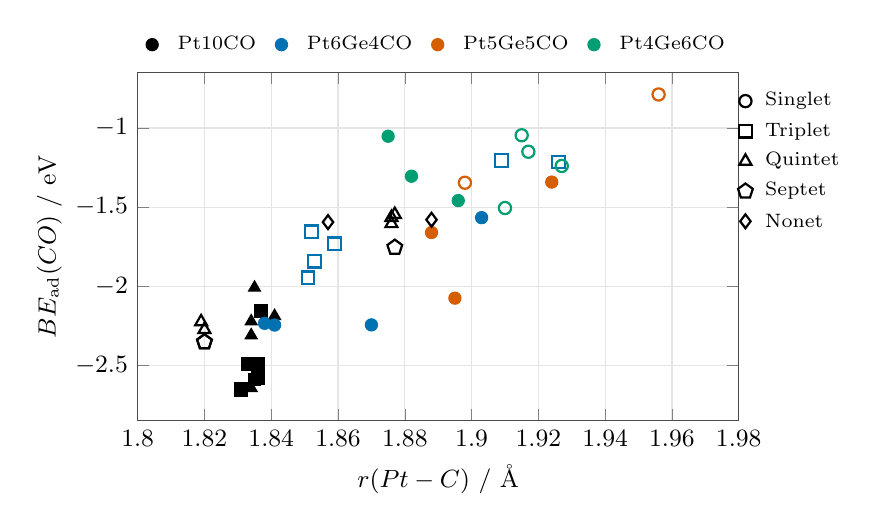
\begin{tikzpicture}
\begin{axis}[
  width=0.76\linewidth,
  height=6.0cm,
  xmin=1.80, xmax=1.98,
  ymin=-2.85, ymax=-0.65,
  xlabel={$r(\ce{Pt-C})$ / \AA},
  ylabel={$BE_{\rm ad}(\ce{CO})$ / eV},
  ylabel style={yshift=-2pt},
  tick label style={font=\small},
  label style={font=\small},
  grid=major,
  grid style={gray!20},
  axis line style={black!70},
  clip=false,
  legend style={at={(0.5,1.03)},anchor=south,draw=none,inner sep=1pt,
    font=\scriptsize,legend columns=4,column sep=5pt}
]
\addlegendimage{only marks,mark=*,mark size=2.2pt,ptten}
\addlegendentry{\ce{Pt10CO}}
\addlegendimage{only marks,mark=*,mark size=2.2pt,ptsixgefour}
\addlegendentry{\ce{Pt6Ge4CO}}
\addlegendimage{only marks,mark=*,mark size=2.2pt,ptfivegefive}
\addlegendentry{\ce{Pt5Ge5CO}}
\addlegendimage{only marks,mark=*,mark size=2.2pt,ptfourgesix}
\addlegendentry{\ce{Pt4Ge6CO}}
% Filled symbols: atom-substitution models.
\addplot[only marks,mark=square*,mark size=2.3pt,ptten] coordinates {
  (1.831,-2.657) (1.831,-2.650) (1.835,-2.590) (1.836,-2.579)
  (1.833,-2.493) (1.836,-2.493) (1.837,-2.156)};
\addplot[only marks,mark=triangle*,mark size=2.5pt,ptten] coordinates {
  (1.834,-2.645) (1.834,-2.311) (1.834,-2.223) (1.841,-2.189)
  (1.835,-2.010)};
\addplot[only marks,mark=*,mark size=2.2pt,ptsixgefour] coordinates {
  (1.841,-2.246) (1.870,-2.245) (1.838,-2.235) (1.903,-1.567)};
\addplot[only marks,mark=*,mark size=2.2pt,ptfivegefive] coordinates {
  (1.895,-2.076) (1.888,-1.661) (1.924,-1.342)};
\addplot[only marks,mark=*,mark size=2.2pt,ptfourgesix] coordinates {
  (1.896,-1.459) (1.882,-1.305) (1.875,-1.052)};
% Open symbols: models initiated from the global-minimum parent.
\addplot[only marks,mark=triangle,mark size=2.5pt,ptten,
  mark options={fill=white,draw=ptten,line width=0.8pt}] coordinates {
  (1.820,-2.275) (1.819,-2.226) (1.876,-1.605) (1.876,-1.566)
  (1.877,-1.547)};
\addplot[only marks,mark=pentagon,mark size=2.8pt,ptten,
  mark options={fill=white,draw=ptten,line width=0.8pt}] coordinates {
  (1.820,-2.353) (1.820,-2.353) (1.877,-1.755)};
\addplot[only marks,mark=diamond,mark size=2.5pt,ptten,
  mark options={fill=white,draw=ptten,line width=0.8pt}] coordinates {
  (1.857,-1.595) (1.888,-1.580)};
\addplot[only marks,mark=square,mark size=2.3pt,ptsixgefour,
  mark options={fill=white,draw=ptsixgefour,line width=0.8pt}] coordinates {
  (1.851,-1.947) (1.853,-1.842) (1.859,-1.732) (1.852,-1.657)
  (1.926,-1.215) (1.909,-1.207)};
\addplot[only marks,mark=o,mark size=2.2pt,ptfivegefive,
  mark options={fill=white,draw=ptfivegefive,line width=0.8pt}] coordinates {
  (1.898,-1.346) (1.956,-0.788)};
\addplot[only marks,mark=o,mark size=2.2pt,ptfourgesix,
  mark options={fill=white,draw=ptfourgesix,line width=0.8pt}] coordinates {
  (1.910,-1.506) (1.927,-1.240) (1.917,-1.150) (1.915,-1.046)};
% Symbol key: fill is reserved for the structural-parent distinction.
\addplot[only marks,mark=o,mark size=2.2pt,black,
  mark options={fill=white,draw=black,line width=0.8pt}] coordinates {(1.982,-0.83)};
\node[anchor=west,font=\scriptsize] at (axis cs:1.985,-0.83) {Singlet};
\addplot[only marks,mark=square,mark size=2.3pt,black,
  mark options={fill=white,draw=black,line width=0.8pt}] coordinates {(1.982,-1.02)};
\node[anchor=west,font=\scriptsize] at (axis cs:1.985,-1.02) {Triplet};
\addplot[only marks,mark=triangle,mark size=2.5pt,black,
  mark options={fill=white,draw=black,line width=0.8pt}] coordinates {(1.982,-1.21)};
\node[anchor=west,font=\scriptsize] at (axis cs:1.985,-1.21) {Quintet};
\addplot[only marks,mark=pentagon,mark size=2.8pt,black,
  mark options={fill=white,draw=black,line width=0.8pt}] coordinates {(1.982,-1.40)};
\node[anchor=west,font=\scriptsize] at (axis cs:1.985,-1.40) {Septet};
\addplot[only marks,mark=diamond,mark size=2.5pt,black,
  mark options={fill=white,draw=black,line width=0.8pt}] coordinates {(1.982,-1.59)};
\node[anchor=west,font=\scriptsize] at (axis cs:1.985,-1.59) {Nonet};
\end{axis}
\end{tikzpicture}

\end{adjustbox}
	\end{center}
\caption{State-specific adiabatic \ce{CO} binding energy versus the optimized
\ce{Pt-C} distance for the carbonyls. Black, blue, vermilion, and green identify \ce{Pt10CO}, \ce{Pt6Ge4CO}, \ce{Pt5Ge5CO}, and \ce{Pt4Ge6CO}, respectively. Filled symbols denote derivative structures and open symbols denote GM structures. Circles, squares, triangles, pentagons, and diamonds represent singlet, triplet, quintet, septet, and nonet states, respectively.}
\label{fig:neutral_be_vs_ptc}
\end{figure}

We next examine the optimized \ce{Pt-C} bond lengths and the electron density at
the bond critical point ($\rho_{\rm BCP}$) to assess how local bonding
descriptors relate to  \(BE_{\rm ad}(\ce{CO})\) \sout{binding strength}\red{puede ser ambiguo yo podría
bindinig energy}. Figure~\textcolor{purple}{\ref{fig:neutral_be_vs_ptc}} reveals a general tendency toward stronger CO binding at shorter \ce{Pt-C} distances, although substantial differences in binding energy are observed even for carbonyls with nearly identical bond lengths.

This behavior is particularly evident for \ce{Pt10^{der}CO}. The triplet minima (black filled squares) exhibit nearly identical \ce{Pt-C} distances (1.83--1.84~\si{\angstromunit}), despite a binding-energy variation of approximately 0.50 eV. A similar trend is observed for the quintet minima (black filled triangles), whose binding energies span 0.64 eV over the same narrow distance range. The GM structures (open symbols\red{simbolos que no tienen relleno}) exhibit a broader distribution of \ce{Pt-C} distances {across different starting geometries and spin states. These differences must also be considered when comparing their binding energies}. The Pt–Ge carbonyls extend the distance range to approximately 1.96~\si{\angstromunit} and provide further evidence that bond length alone does not determine adsorption strength. For instance, sites 6/8 and 7/10 of \ce{Pt5Ge5^{der}CO} have similar \ce{Pt-C} distances (1.90 and 1.89~\si{\angstromunit}), yet their binding energies differ by 0.42 eV ($-2.08$ and $-1.66$ eV, respectively).

The AIM analysis provides a complementary measure of local \ce{Pt-C} bonding through $\rho_{\rm BCP}$ (Table~\ref{tab:tfg_interaction_deformation}). For the selected strongest- and weakest-binding sites of \ce{Pt10}, \ce{Pt6Ge4}, and \ce{Pt5Ge5} (6 versus 1/9, 2 versus 5/7, and 6/8 versus 4, respectively), stronger CO binding is accompanied by higher $\rho_{\rm BCP}$. However, this correlation is not universal. Sites 6/8 and 7/10 of \ce{Pt5Ge5} exhibit nearly identical electron densities (0.173 and 0.175 \sout{$e,a_0^{-3}$}\textcolor{purple}{$e\,a_0^{-3}$}), despite their 0.42 eV binding-energy difference. Likewise, site 1 of \ce{Pt4Ge6} has a higher $\rho_{\rm BCP}$ than site 5/7 (0.181 versus 0.171 {$e\,a_0^{-3}$}), yet binds CO more weakly.

These examples show that the \ce{Pt-C} distance and $\rho_{\rm BCP}$ describe aspects of the local bond, while the binding energy also reflects the interaction and structural reorganization of the cluster. The fragment-energy analysis in Section~\ref{subsec:interaction_fragment_reorganization} examines these contributions.



To complement the ECoN analysis, we decompose the electronic CO binding energy
into the frozen-fragment interaction and the energy changes associated with
metal-cluster and CO reorganization. A similar approach was employed by Gasper
\textit{et al.} to investigate CO adsorption on Pt clusters. They found that the \ce{CO}--Pt interaction was the
main contribution to adsorption, with a smaller contribution from
cluster relaxation\cite{gasper:2017}

\subsubsection{Energy decomposition and \ce{Pt10} comparison}
\label{subsec:interaction_fragment_reorganization}

We first consider three triplet \ce{Pt10^{der}CO} minima obtained from the same
bare-cluster structure: the strongest-binding minimum reached from site 6, the
weakest-binding minimum reached from sites 1/9, and the minimum reached from
sites 8/10. For each optimized carbonyl, the interaction energy is calculated using the isolated metal and CO fragments frozen at their geometries in the complex:

\begin{align}
E_{\mathrm{int}} &=
E_{\ce{Pt10CO}}(\mathbf R_{\ce{Pt10CO}})
-E_{\ce{Pt10}}(\mathbf R_{\ce{Pt10}}^{\ce{Pt10CO}})
-E_{\ce{CO}}(\mathbf R_{\ce{CO}}^{\ce{Pt10CO}}),\\
E_{\mathrm{def}} &=
\left[
E_{\ce{Pt10}}(\mathbf R_{\ce{Pt10}}^{\ce{Pt10CO}})
-E_{\ce{Pt10}}(\mathbf R_{\ce{Pt10}}^{0})
\right]
{}+
\left[
E_{\ce{CO}}(\mathbf R_{\ce{CO}}^{\ce{Pt10CO}})
-E_{\ce{CO}}(\mathbf R_{\ce{CO}}^{0})
\right],
\label{eq:tfg_deformation}
\end{align}

where $\mathbf R^{\ce{Pt10CO}}$ denotes the fragment geometry in the optimized carbonyl, while $\mathbf R^0$ refers to the corresponding isolated reference structure (\ce{Pt10^{der}} or singlet \ce{CO}). {The same bare-cluster reference, \ce{Pt10^{der}}, is used for all three carbonyl complexes.} The two contributions to $E_{\rm def}$ are denoted $E_{\rm reorg}^{\rm metal}$      and $E_{\rm reorg}^{\ce{CO}}$, respectively. Thus, $\Delta E_{\rm elec}=E_{\rm int}+E_{\rm def}$, where $\Delta E_{\rm elec}$ is the electronic binding energy before the ZPVE correction. The zero-point vibrational correction is subsequently added to obtain $BE_{\rm ad}(\ce{CO})$.

{The reorganization terms measure the energy change from each optimized isolated reference to the frozen fragment geometry in the carbonyl. Positive values indicate destabilization relative to that reference, and negative values indicate stabilization. A negative metal term therefore means that the isolated metal fragment at its carbonyl complex geometry has a lower electronic energy than the selected bare-cluster reference.}

For \ce{Pt10^{der}CO}, the strongest-binding site 6 exhibits a frozen-fragment interaction of $-2.71$ eV and a slightly stabilizing metal-reorganization contribution of $-0.06$ eV. In contrast, the weakest-binding minimum (sites 1/9) has a less favorable interaction ($-2.46$ eV) and a positive metal-reorganization contribution ($0.20$ eV). {Including the small CO-reorganization contribution listed in Table~\ref{tab:tfg_interaction_deformation}, $\Delta E_{\rm elec}$ is $-2.74$ eV for site 6 and $-2.24$ eV for sites 1/9.} Thus, the 0.50 eV difference in electronic binding energy arises from both a stronger interaction (0.25 eV) and more favorable metal reorganization (0.26 eV) at site 6. The minimum reached from sites 8/10 exhibits similar binding energies and decomposition terms to site 6 (Table~\textcolor{purple}{\ref{tab:tfg_interaction_deformation}}).

Since the CO-reorganization contribution is small and nearly constant across the
selected carbonyls (0.02–0.03 eV), the following discussion focuses on the 
contributions
from frozen-fragment interaction and metal-cluster reorganization.

\subsubsection{Interaction and reorganization in Pt--Ge clusters}
\label{subsec:ptge_interaction_reorganization}

{We applied the same analysis to
selected strong- and weak CO-binding minima of the three Pt--Ge derivatives. We
also compared sites 6/8 and 7/10 of \ce{Pt5Ge5^{der}CO}, which have similar
initial $x_{\rm Ge}^{0}$ values but different total ECoN and binding energies
(Table~\ref{tab:tfg_interaction_deformation}).}

For \ce{Pt6Ge4^{der}}, the 0.68 eV stronger $BE_{\rm ad}(\ce{CO})$ at site 2 is mainly associated with its more stabilizing frozen-fragment interaction, which is 0.79 eV more favorable than at site 5/7. Its metal-reorganization term is 0.08 eV less favorable, which slightly reduces this advantage. The lower $x_{\rm Ge}^{0}$ at site 2 is consistent with its stronger binding. However, site 2 also has a higher $ECoN_{\rm total}^{0}$ than site 5/7 and still binds \ce{CO} more strongly, contrary to the expectation based on lower coordination. The fragment terms show that the difference in binding energy is mainly associated with $E_{\rm int}$.

Similarly, in \ce{Pt4Ge6^{der}}, sites 5/7 bind CO 0.41 eV more strongly than site 1, with both the interaction ($-1.89$ versus $-1.66$ eV) and metal reorganization (0.34 versus 0.52 eV) favoring sites 5/7. These results indicate that, while the frozen-fragment interaction plays a major role in both compositions, metal reorganization can either reinforce or partially compensate for differences in interaction strength. Both contributions therefore account for the stronger binding at sites 5/7. The initial ECoN descriptors show that site 1 has a larger $x_{\rm Ge}^{0}$ (0.98 versus 0.86 and 0.92) and a higher $ECoN_{\rm total}^{0}$ (4.41 versus 3.99 for site 5 and 3.48 for site 7). The weaker binding at site 1 is consistent with both its larger initial Ge fraction and its higher initial total coordination compared with sites 5/7.

\sout{A markedly different behavior emerges for \ce{Pt5Ge5^{der}}, where metal reorganization becomes the dominant factor.} \red{Me parece demasiado IA} \blue{Algo asi: A completely different behavior is observed in \ce{Pt5Ge5^{der}}, where metal reorganization is the dominant factor.} {Site 6/8 binds \ce{CO} 0.74 eV more strongly than site 4. The metal-reorganization term is $-0.40$ eV for site 6/8 and 0.49 eV for site 4, favoring site 6/8 by 0.89 eV. The frozen-fragment interaction favors site 4 by only 0.14 eV ($-1.92$ versus $-1.78$ eV). The larger difference in metal reorganization therefore gives stronger \ce{CO} binding at site 6/8. The lower initial $x_{\rm Ge}^{0}$ at site 6/8 (0.75 versus 1.00) is consistent with its stronger binding, even though this site is initially more highly coordinated ($ECoN_{\rm total}^{0}=5.58$ versus 2.95).}

\textcolor{ForestGreen}{\sout{The ECoN analysis in Section~\ref{subsec:local_pt_coordination} showed that sites 6/8 and 7/10 of \ce{Pt5Ge5^{der}} have almost identical $x_{\rm Ge}^{0}$ values (0.75 at both sites), but different $ECoN_{\rm total}^{0}$ values (5.58 and 2.91) and $BE_{\rm ad}(\ce{CO})$ values ($-2.08$ and $-1.66$ eV, respectively). $ECoN_{\rm total}^{0}$ sums the effective contributions from Pt and Ge neighbors. Its higher value for site 6/8 indicates a more highly coordinated initial Pt environment, while the similar $x_{\rm Ge}^{0}$ values show that the relative Ge contribution is nearly the same at both sites. Lower initial coordination would suggest stronger binding at site 7/10, whereas site 6/8 binds \ce{CO} more strongly by 0.42 eV. To examine this, we compare the fragment-energy contributions for the two minima, separating the interaction at the optimized carbonyl geometries from the energy changes associated with fragment reorganization.}}\textcolor{purple}{We return to sites 6/8 and 7/10 of \ce{Pt5Ge5^{der}}, discussed in Section~\ref{subsec:local_pt_coordination}, because their similar initial Ge fractions do not explain their different binding energies. The fragment contributions identify the energetic origin of this difference.} Site 7/10 has a more stabilizing frozen-fragment interaction than site 6/8 ($-1.92$ versus $-1.78$ eV), but its metal-reorganization term is positive ($0.17$ eV), whereas that of site 6/8 is stabilizing ($-0.40$ eV). This difference in metal reorganization is larger than the interaction advantage of site 7/10. As a result, the electronic binding energy is less negative for site 7/10 ($-1.73$ versus $-2.15$ eV), consistent with the final $BE_{\rm ad}(\ce{CO})$ values ($-1.66$ versus $-2.08$ eV).

\begin{table}[htbp]
\caption{{Interaction and fragment-reorganization terms for selected
\ce{CO}-binding minima obtained from the derivative models. All
decomposed terms use electronic energies and are reported in eV. The \ce{Pt10}
entries are triplets and the Pt--Ge entries are singlets.
Each bare-cluster reference is the selected optimized
structure used for the corresponding binding energy, with the same
multiplicity as the carbonyl.The final $BE_{\rm ad}(\ce{CO})$ column includes the
zero-point correction. The $\rho_{\rm BCP}$ column gives the electron density
at the Pt--C bond critical point of each optimized carbonyl, in $e\,a_0^{-3}$. A
negative metal-reorganization term means that the metal fragment is stabilized
at the geometry it adopts in the carbonyl, relative to the selected optimized
bare-cluster reference.}}
\label{tab:tfg_interaction_deformation}
%\scriptsize
\begin{adjustbox}{max width=\linewidth}
\begin{tabular}{lclrrrrrr}
\toprule
{System} & {$2S+1$} & {Site(s)} & {$\Delta E_{\rm elec}$} &
{$E_{\rm int}$} & {$E_{\rm reorg}^{\rm metal}$} &
{$E_{\rm reorg}^{\ce{CO}}$} & {$BE_{\rm ad}(\ce{CO})$} &
{$\rho_{\rm BCP}$} \\
\midrule
\ce{Pt10} & 3 & 6   & -2.74 & -2.71 & -0.06 & 0.03 & -2.66 & 0.199 \\
{\ce{Pt10}} & {3} & {8/10} & {-2.73} & {-2.79} & {0.03} & {0.03} & {-2.65} & {0.198} \\
\ce{Pt10} & 3 & 1/9 & -2.24 & -2.46 &  0.20 & 0.02 & -2.16 & 0.196 \\
\midrule
\ce{Pt6Ge4^{der}} & 1 & 2   & -2.33 & -2.70 &  0.35 & 0.03 & -2.25 & 0.194 \\
\ce{Pt6Ge4^{der}} & 1 & 5/7 & -1.63 & -1.91 &  0.27 & 0.02 & -1.57 & 0.182 \\
\midrule
\ce{Pt5Ge5^{der}} & 1 & 6/8 & -2.15 & -1.78 & -0.40 & 0.02 & -2.08 & 0.173 \\
\ce{Pt5Ge5^{der}} & 1 & 7/10 & -1.73 & -1.92 &  0.17 & 0.02 & -1.66 & 0.175 \\
\ce{Pt5Ge5^{der}} & 1 & 4   & -1.41 & -1.92 &  0.49 & 0.02 & -1.34 & 0.162 \\
\midrule
\ce{Pt4Ge6^{der}} & 1 & 5/7 & -1.53 & -1.89 &  0.34 & 0.02 & -1.46 & 0.171 \\
\ce{Pt4Ge6^{der}} & 1 & 1   & -1.12 & -1.66 &  0.52 & 0.02 & -1.05 & 0.181 \\
\bottomrule
\end{tabular}
\end{adjustbox}

\end{table}

Although lower coordination often favors \ce{CO} binding on Pt nanoparticles,\cite{hossain:lowcoord:2020} the Pt--Ge cluster examples show that the local Ge fraction and metal-cluster reorganization also affect the binding-energy order. \textcolor{ForestGreen}{\sout{Taken together, these results show that the calculated $BE_{\rm ad}(\ce{CO})$ depends on several effects. The frozen-fragment interaction and metal-cluster reorganization contribute in different proportions across sites and compositions. ECoN describes the initial Pt environment, while the fragment analysis shows how interaction and structural reorganization combine in the final binding energy.}}\textcolor{purple}{Across these selected cases, the binding-energy differences reflect different balances between frozen-fragment interaction and metal-cluster reorganization.}
